% This is the Reed College LaTeX thesis template. Most of the work
% for the document class was done by Sam Noble (SN), as well as this
% template. Later comments etc. by Ben Salzberg (BTS). Additional
% restructuring and APA support by Jess Youngberg (JY).
% Your comments and suggestions are more than welcome; please email
% them to cus@reed.edu
%
% See http://web.reed.edu/cis/help/latex.html for help. There are a
% great bunch of help pages there, with notes on
% getting started, bibtex, etc. Go there and read it if you're not
% already familiar with LaTeX.
%
% Any line that starts with a percent symbol is a comment.
% They won't show up in the document, and are useful for notes
% to yourself and explaining commands.
% Commenting also removes a line from the document;
% very handy for troubleshooting problems. -BTS

% As far as I know, this follows the requirements laid out in
% the 2002-2003 Senior Handbook. Ask a librarian to check the
% document before binding. -SN

%%
%% Preamble
%%
% \documentclass{<something>} must begin each LaTeX document
\documentclass[12pt,twoside]{reedthesis}
% Packages are extensions to the basic LaTeX functions. Whatever you
% want to typeset, there is probably a package out there for it.
% Chemistry (chemtex), screenplays, you name it.
% Check out CTAN to see: http://www.ctan.org/
%%
\usepackage{graphicx,latexsym}
\usepackage{amsmath}
\usepackage{amssymb,amsthm}
\usepackage{longtable,booktabs,setspace}
\usepackage{chemarr} %% Useful for one reaction arrow, useless if you're not a chem major
\usepackage[hyphens]{url}
% Added by CII
\usepackage{hyperref}
\usepackage{lmodern}
\usepackage{float}
\floatplacement{figure}{H}
% End of CII addition
\usepackage{rotating}

% Next line commented out by CII
%%% \usepackage{natbib}
% Comment out the natbib line above and uncomment the following two lines to use the new
% biblatex-chicago style, for Chicago A. Also make some changes at the end where the
% bibliography is included.
%\usepackage{biblatex-chicago}
%\bibliography{thesis}


% Added by CII (Thanks, Hadley!)
% Use ref for internal links
\renewcommand{\hyperref}[2][???]{\autoref{#1}}
\def\chapterautorefname{Chapter}
\def\sectionautorefname{Section}
\def\subsectionautorefname{Subsection}
% End of CII addition

% Added by CII
\usepackage{caption}
\captionsetup{width=5in}
% End of CII addition

% \usepackage{times} % other fonts are available like times, bookman, charter, palatino

% Syntax highlighting #22
  \usepackage{color}
  \usepackage{fancyvrb}
  \newcommand{\VerbBar}{|}
  \newcommand{\VERB}{\Verb[commandchars=\\\{\}]}
  \DefineVerbatimEnvironment{Highlighting}{Verbatim}{commandchars=\\\{\}}
  % Add ',fontsize=\small' for more characters per line
  \usepackage{framed}
  \definecolor{shadecolor}{RGB}{248,248,248}
  \newenvironment{Shaded}{\begin{snugshade}}{\end{snugshade}}
  \newcommand{\AlertTok}[1]{\textcolor[rgb]{0.94,0.16,0.16}{#1}}
  \newcommand{\AnnotationTok}[1]{\textcolor[rgb]{0.56,0.35,0.01}{\textbf{\textit{#1}}}}
  \newcommand{\AttributeTok}[1]{\textcolor[rgb]{0.77,0.63,0.00}{#1}}
  \newcommand{\BaseNTok}[1]{\textcolor[rgb]{0.00,0.00,0.81}{#1}}
  \newcommand{\BuiltInTok}[1]{#1}
  \newcommand{\CharTok}[1]{\textcolor[rgb]{0.31,0.60,0.02}{#1}}
  \newcommand{\CommentTok}[1]{\textcolor[rgb]{0.56,0.35,0.01}{\textit{#1}}}
  \newcommand{\CommentVarTok}[1]{\textcolor[rgb]{0.56,0.35,0.01}{\textbf{\textit{#1}}}}
  \newcommand{\ConstantTok}[1]{\textcolor[rgb]{0.00,0.00,0.00}{#1}}
  \newcommand{\ControlFlowTok}[1]{\textcolor[rgb]{0.13,0.29,0.53}{\textbf{#1}}}
  \newcommand{\DataTypeTok}[1]{\textcolor[rgb]{0.13,0.29,0.53}{#1}}
  \newcommand{\DecValTok}[1]{\textcolor[rgb]{0.00,0.00,0.81}{#1}}
  \newcommand{\DocumentationTok}[1]{\textcolor[rgb]{0.56,0.35,0.01}{\textbf{\textit{#1}}}}
  \newcommand{\ErrorTok}[1]{\textcolor[rgb]{0.64,0.00,0.00}{\textbf{#1}}}
  \newcommand{\ExtensionTok}[1]{#1}
  \newcommand{\FloatTok}[1]{\textcolor[rgb]{0.00,0.00,0.81}{#1}}
  \newcommand{\FunctionTok}[1]{\textcolor[rgb]{0.00,0.00,0.00}{#1}}
  \newcommand{\ImportTok}[1]{#1}
  \newcommand{\InformationTok}[1]{\textcolor[rgb]{0.56,0.35,0.01}{\textbf{\textit{#1}}}}
  \newcommand{\KeywordTok}[1]{\textcolor[rgb]{0.13,0.29,0.53}{\textbf{#1}}}
  \newcommand{\NormalTok}[1]{#1}
  \newcommand{\OperatorTok}[1]{\textcolor[rgb]{0.81,0.36,0.00}{\textbf{#1}}}
  \newcommand{\OtherTok}[1]{\textcolor[rgb]{0.56,0.35,0.01}{#1}}
  \newcommand{\PreprocessorTok}[1]{\textcolor[rgb]{0.56,0.35,0.01}{\textit{#1}}}
  \newcommand{\RegionMarkerTok}[1]{#1}
  \newcommand{\SpecialCharTok}[1]{\textcolor[rgb]{0.00,0.00,0.00}{#1}}
  \newcommand{\SpecialStringTok}[1]{\textcolor[rgb]{0.31,0.60,0.02}{#1}}
  \newcommand{\StringTok}[1]{\textcolor[rgb]{0.31,0.60,0.02}{#1}}
  \newcommand{\VariableTok}[1]{\textcolor[rgb]{0.00,0.00,0.00}{#1}}
  \newcommand{\VerbatimStringTok}[1]{\textcolor[rgb]{0.31,0.60,0.02}{#1}}
  \newcommand{\WarningTok}[1]{\textcolor[rgb]{0.56,0.35,0.01}{\textbf{\textit{#1}}}}

% To pass between YAML and LaTeX the dollar signs are added by CII
\title{My Final College Paper}
\author{Your R. Name}
% The month and year that you submit your FINAL draft TO THE LIBRARY (May or December)
\date{May 20xx}
\division{Mathematics and Natural Sciences}
\advisor{Advisor F. Name}
\institution{Reed College}
\degree{Bachelor of Arts}
%If you have two advisors for some reason, you can use the following
% Uncommented out by CII
% End of CII addition

%%% Remember to use the correct department!
\department{Mathematics}
% if you're writing a thesis in an interdisciplinary major,
% uncomment the line below and change the text as appropriate.
% check the Senior Handbook if unsure.
%\thedivisionof{The Established Interdisciplinary Committee for}
% if you want the approval page to say "Approved for the Committee",
% uncomment the next line
%\approvedforthe{Committee}

% Added by CII
%%% Copied from knitr
%% maxwidth is the original width if it's less than linewidth
%% otherwise use linewidth (to make sure the graphics do not exceed the margin)
\makeatletter
\def\maxwidth{ %
  \ifdim\Gin@nat@width>\linewidth
    \linewidth
  \else
    \Gin@nat@width
  \fi
}
\makeatother

\renewcommand{\contentsname}{Table of Contents}
% End of CII addition

\setlength{\parskip}{0pt}

% Added by CII

\providecommand{\tightlist}{%
  \setlength{\itemsep}{0pt}\setlength{\parskip}{0pt}}

\Acknowledgements{
I want to thank a few people.
}

\Dedication{
You can have a dedication here if you wish.
}

\Preface{
This is an example of a thesis setup to use the reed thesis document class
(for LaTeX) and the R bookdown package, in general.
}

\Abstract{
The preface pretty much says it all.

\par

Second paragraph of abstract starts here.
}

% End of CII addition
%%
%% End Preamble
%%
%
\begin{document}

% Everything below added by CII
  \maketitle

\frontmatter % this stuff will be roman-numbered
\pagestyle{empty} % this removes page numbers from the frontmatter
  \begin{acknowledgements}
    I want to thank a few people.
  \end{acknowledgements}
  \begin{preface}
    This is an example of a thesis setup to use the reed thesis document class
    (for LaTeX) and the R bookdown package, in general.
  \end{preface}
  \hypersetup{linkcolor=black}
  \setcounter{tocdepth}{2}
  \tableofcontents

  \listoftables

  \listoffigures
  \begin{abstract}
    The preface pretty much says it all.
    
    \par
    
    Second paragraph of abstract starts here.
  \end{abstract}
  \begin{dedication}
    You can have a dedication here if you wish.
  \end{dedication}
\mainmatter % here the regular arabic numbering starts
\pagestyle{fancyplain} % turns page numbering back on

\hypertarget{introduction}{%
\chapter*{Introduction}\label{introduction}}
\addcontentsline{toc}{chapter}{Introduction}

\hypertarget{background}{%
\section*{Background}\label{background}}
\addcontentsline{toc}{section}{Background}

Starting from the second half of the 20th century, the development of high technologies in various industries and the production of a fundamentally new high-tech products have become critical factors in sustainable economic growth for most industrialized countries of the world. The rapid development of science and technology, global political and technological transformations led to dramatic changes in the international economic system, and in the XXI century, the world economy entered a new phase of its development, turning into a knowledge economy, the main driving force of which was knowledge-intensive technology. Most of these tendencies are changing the future of the companies, operation in the automotive industry.

The relevance of the study is emerging due to economic problems in the development of scientific and production enterprises of the automotive industry under intense-changing prevailing conditions happening on the market. The specifics of the activities of these enterprises is the need for a rational combination and balanced development of automotive equipment and technologies used, specifically in the interests of strengthening competitive positions in the international market of automotive and logistics services by commercializing the results of Research and Development (R\&D) outcomes as part of the implementation of business agreements between interested parties.

Apparently, the cost-effective functioning of automotive industry enterprises is possible due to the strategic planning of R\&D, taking into account the potential of innovation and commercialization of the created technologies in the entrepreneurial sector of the economy. The most crucial tool for strategic planning of R\&D is prospective patent research. Based on the forecast of development trends of scientific and technical areas and objects of technology, it allows us to substantiate target criteria for efficiency and product requirements and evaluate its technical level. Prospective patent research also supports the generation of competitive intellectual property objects, which directly affects the economic efficiency of R\&D results, since intellectual property forms the bulk of the added value of high-tech products and provides revenue from the sale of patents and licenses.

The purpose of the thesis is to develop an organizational and economic mechanism for prospective patent research, which will increase the economic efficiency of fleet industry enterprises. Formed on the analysis of the features of the fleet management industry and the existing approaches to strategic planning of R\&D, it is proposed to solve the scientific task of developing an organizational and economic mechanism for promising patent research as a tool for strategic planning of R\&D's in fleet management companies, following technological diversification and marketing trends. The research aims not only connect intricate conceptual part of new potential business model approaches for the fleet management organizations but also to develop a forecast model by received of system-forming techniques for the organizational and economic mechanism of promising patent research.

Fleet management is considering as an area of logistics and transportation utilities, where companies are retransferring a series of procedures to fleet companies, including integrated outsourcing, operational leasing, and the possibilities of corporate rental, maintenance, and insurance. Due to technological changes, innovative devices implementation, and a new paradigm in methodologies for solving route problems in vehicle transportation, there is a emerge need to formulate a retrospective analysis of current trends in fleet management. An efficient operational system is vital for each state of the company's implementation and development process, varying from fleet tracking software to management changes for reducing operational costs. Thus, by studying the specific cases of technology forecasting and modeling principles, this work investigates the use of these technologies in the management of workflow and services through patent data acquisition models.

Therefore, to explain the issues mentioned before and achieve a complete understanding, there is an emerging necessity to answer the following questions. The overall process can be represented in 4 main research questions (RQ) as an analytical basis for the research; the following central questions are:

\textbf{RQ1:}
\emph{What are the current tendencies for data-driven businesses (acquisition of data) and technology innovations in local solutions, transport management system (TMS) and fleet management (FM)?}

\textbf{RQ2:}
\emph{How can companies, operating in the fleet management context benefit from utilizing existing datasets and enhance practical business model ecosystem trough benchmarking and patent analysis?}

\textbf{RQ3:}
\emph{Based on patent analytics, in what areas a company should forecast and predict to see disruptive innovations in fleet management?}

\textbf{RQ4:}
\emph{What are the main predictors and and how we can forecast indicators for future scenario changes in fleet management?}

Technical literature, statistics, case studies, and patent information extracted from multiple sources were used for central research issues, defined goals, and duties. The publications of periodicals and magazines were implemented in order to provide topicality information highly.

\hypertarget{research-outline}{%
\section*{Research outline}\label{research-outline}}
\addcontentsline{toc}{section}{Research outline}

\hypertarget{research-scope}{%
\section*{Research scope}\label{research-scope}}
\addcontentsline{toc}{section}{Research scope}

\hypertarget{literature-review}{%
\chapter{Literature review}\label{literature-review}}

\hypertarget{tms-fms-and-rda-system}{%
\section{TMS, FMS and RDA system}\label{tms-fms-and-rda-system}}

The following three groups of solutions can be distinguished according to the software market for the automation of transportation processes. Figure \ref{fig:tmssystems} representing categories of transportation management information systems (Griffis \& Goldsby, 2007; ``Which one is for you,'' 2019).
\begin{Shaded}
\begin{Highlighting}[]
\KeywordTok{include_graphics}\NormalTok{(}\StringTok{"figure/all_systems.pdf"}\NormalTok{)}
\end{Highlighting}
\end{Shaded}
\begin{figure}[h]

{\centering 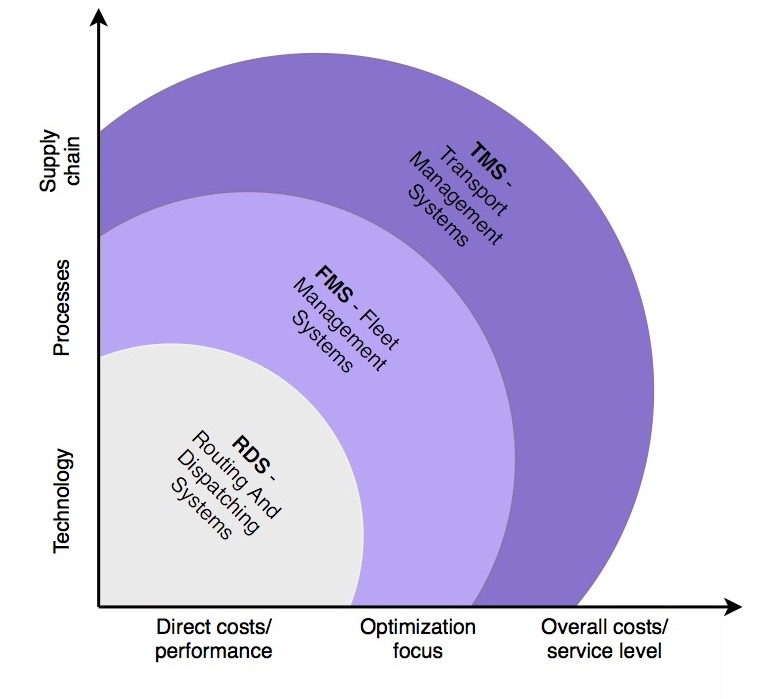
\includegraphics[width=0.9\linewidth,]{figure/all_systems} 

}

\caption{The main categories of information systems for managing transportation processes (Source: Personal drawings)}\label{fig:tmssystems}
\end{figure}
\begin{enumerate}
\def\labelenumi{\arabic{enumi}.}
\tightlist
\item
  Local solutions - software products that automate individual tasks as part of a continuous transportation process (optimization of vehicle loading, route planning, scheduling, calculation of transportation tariffs).
\end{enumerate}
This category of software products includes transport routing and dispatching systems - a combination of technical means (navigation and communication equipment, sensors), data transmission channels and software for monitoring key performance indicators and operational vehicle management.

Through such systems users can track multiple vehichle paramets, such as on/off-line control of speed, route, driving schedules, mileage and fuel consumption, control of vehicle operation modes (idle time, at high engine speeds, status of the brake pedal and clutch), control of the main parameters the operation of vehicle systems (engine temperature, fuel pressure, on-board voltage, malfunction indicator lamps, engine coolant temperature, fuel temperature, engine oil pressure, torque engine entrant, load on the vehicle's axles), monitoring the temperature of cargo transportation, monitoring the location of vehicles, cargo, drivers, monitoring the execution of route tasks with an alarm about their violation.

Routing and dispatching systems of transport allow you to implement a full cycle of vehicle management at the operational level:
\begin{itemize}
\tightlist
\item
  Assign route tasks manually or automatically according to a specified work schedule
\item
  Track the progress of the route task (determining the location, direction of movement, passing the ``control'' points - performing certain operations - time and place of loading / unloading of goods)
\item
  Determine the condition of the vehicle, the operation of special systems and equipment based on sensor readings
\item
  Quickly change route tasks during execution
\item
  Generate reports on the movement of vehicles, use of working time, forming a statistical base for subsequent analysis and optimization of transportation processes
\end{itemize}
\begin{enumerate}
\def\labelenumi{\arabic{enumi}.}
\setcounter{enumi}{1}
\tightlist
\item
  In the conditions of a dynamic market and fierce competition, companies seek ways to reduce costs and minimize expenditure on the material base. Thus, most enterprises use motor transport in their activities and, among other things, car fleet outsourcing becomes one of the ways to optimize costs. The concept of fleet management refers to a range of services, which involves the transfer of its vehicle fleet pool to external management, in order to ensure efficient operation and optimize the cost of its maintenance. Besides standard practices, there is also another type of fleet outsourcing - operational leasing. Outsourcing (use of external sources) is the transfer to an outside organization of tasks, business functions or business processes that are not the main activity of the company, but are necessary for the full functioning of the business (Twin, n.d.). Fleet management is a complex of services that provides for the transfer of its own fleet to external management in order to ensure efficient operation and optimize the cost of its maintenance (``What is fleet management?'' n.d.). Figure \ref{fig:fleetmanagementsystem} showing the outline schematic of fleet management.
\end{enumerate}
\begin{Shaded}
\begin{Highlighting}[]
\KeywordTok{include_graphics}\NormalTok{(}\StringTok{"figure/fleetmanagementsystem.pdf"}\NormalTok{)}
\end{Highlighting}
\end{Shaded}
\begin{figure}[h]

{\centering 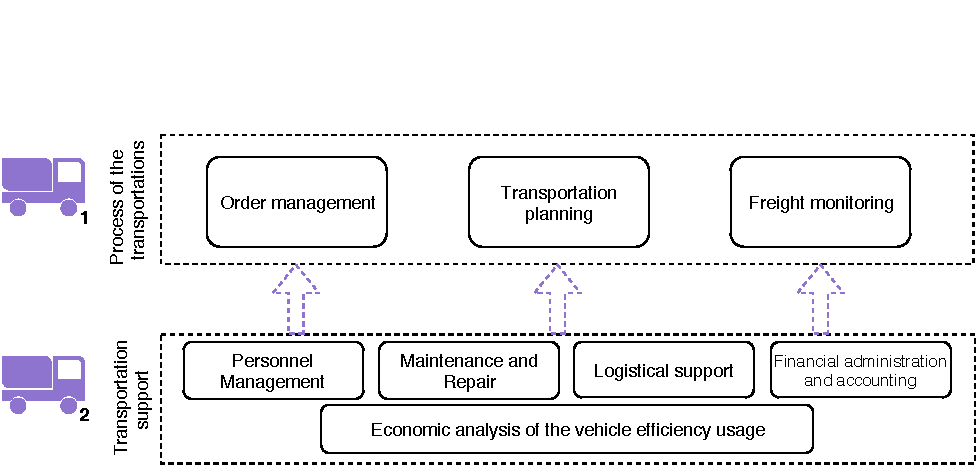
\includegraphics[width=0.9\linewidth,]{figure/fleetmanagementsystem} 

}

\caption{Fleet management. (Source: Personal drawings)}\label{fig:fleetmanagementsystem}
\end{figure}
A distinctive feature of this type of solution is the creation of a centralized transportation plan: on the basis of order data (internal or external), the system can select the necessary type of transport and a specific vehicle, taking into account the characteristics of the vehicle (for example, data on the average consumption of fuels and lubricants - for planning gas stations and related time and financial costs) and features of routes, already issued tasks, requirements of an external / internal customer, ha akteristik cargo. The criteria for optimizing the transportation plan may be loading the vehicle, and minimizing the cost of transportation, reducing downtime or empty vehicle mileage, etc. When planning, measures for maintenance and repair of vehicles are also taken into account. It also supports the management of the fleet of vehicles as capital assets (support of transactions for the acquisition of a vehicle into ownership, leasing, rental, commissioning / withdrawal of a vehicle from/to operation, vehicle insurance, depreciation and change in the value of the vehicle in connection with the maintenance and repairs, revaluation, operating costs management).

Operational leasing is a financing instrument that opens up great opportunities for business development. The leasing service scheme allows you to purchase vehicles or special equipment for a specified period without using the working capital (current assets) of the company. Upon expiration of the contract, the leased asset is returned to the leasing company, or it can be purchased at a residual value of approximately 30--40\% of the original. The advantages of operating leasing include the following features:
\begin{itemize}
\item
  Optimization of tax payments. The lessee can consider the expenses of the leasing company payments, therefore limiting tax base and as well as reimburse value-added tax (VAT) on payments being already made.
\item
  Operational leasing, like others forms, allows you to receive equipment or machines radpidly. The registration duties are the responsibilities of the lessor, as further maintenance and insurance.
\item
  All financial risks are borne by the landlord, as a result of which the client becomes protected from unforeseen expenses.
\item
  In fact, when concluding an operating lease agreement, the tenant is able to pay only for the use of the vechicle. When the contract ends, the car will be returned to the owner, and the amount of all leasing payments is reduced by the residual value of the vechile cost price.
\end{itemize}
The outsourcing company develops fleet management programs individually for each corporate client, taking into account its requirements and business specifics, analyzing all customer expense items, offers ways to optimize and improves the fleet management system. The experience and professionalism of the outsourcer provide a quick solution to current problems within the framework of the customer's corporate policy, cost effectiveness and maximum financial transparency. A full range of fleet management services contains many options, you can choose your specific services, which is relevant to particlular business. In this case, the customer receives regular reports on the operation of the fleet. According to the ReportBuyer (n.d.) there are emerging amount of passenger vehicles and LCV in Finland, exceeding over 66,000 leased vehicles by the end of 2014.
\begin{enumerate}
\def\labelenumi{\arabic{enumi}.}
\setcounter{enumi}{2}
\tightlist
\item
  Transport Management (TMS) System has historically evolved from fragmented solutions to end-to-end transportation process management in the value chain within a single platform that integrates various automation applications for transportation management tasks into a single information system. The implementation of TMS is focused on increasing the adaptability and productivity of transportation processes, reducing costs and increasing the level of service in the supply chain (Griffis \& Goldsby, 2007; Nettsträter, Geißen, Witthaut, Ebel, \& Schoneboom, 2015). Regarding the Muynck (2018) and Brock Johns (n.d.) - Transportation Management Systems (TMS) are considered to be part of the Supply Chain Management (SCM) class of systems, which, in turn, are part of Enterprise Resource Planning (ERP) systems. More presicely the connections between major systems is delighted in the works of Nettsträter et al. (2015) and Figure \ref{fig:tmscomplexity} showing principles related.
\end{enumerate}
\begin{Shaded}
\begin{Highlighting}[]
\KeywordTok{include_graphics}\NormalTok{(}\StringTok{"figure/TMScomplexity.pdf"}\NormalTok{)}
\end{Highlighting}
\end{Shaded}
\begin{figure}[h]

{\centering 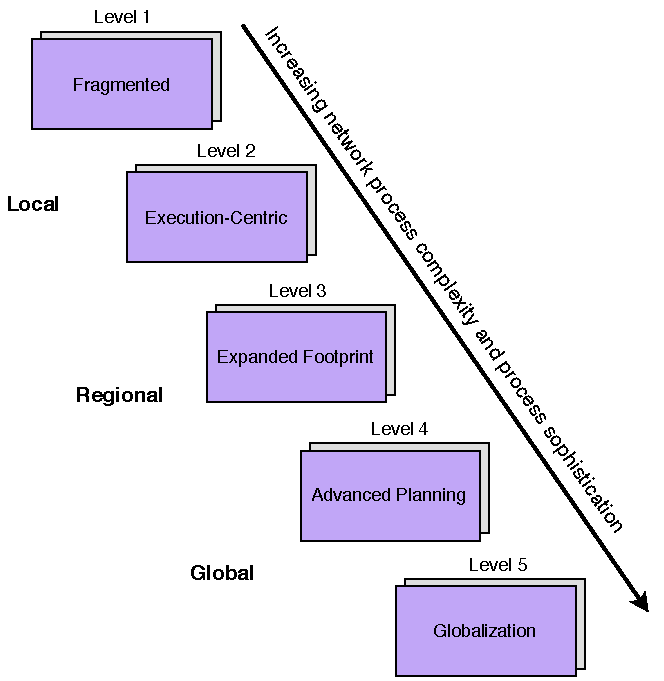
\includegraphics[width=0.9\linewidth,]{figure/TMScomplexity} 

}

\caption{Levels of TMS complexity according to Garter (2019)}\label{fig:tmscomplexity}
\end{figure}
Transportation management systems is a comprehensive solution that covers the entire transportation process from supporting strategic decision-making procedures, procurement planning and scheduling of transport to delivery and monitoring, cost management and coordination with consumers and providers of transport services. Often TMS-systems act as a separate business application, but the greatest effect is achieved when they are integrated with other subsystems of global products such as ERP or SCM-systems (Wiyono, Pribadi, \& Permana, 2011). The place for the TMS in the Supply Chain Management Information System can be represented in the Figure \ref{fig:tms}.
\begin{Shaded}
\begin{Highlighting}[]
\KeywordTok{include_graphics}\NormalTok{(}\StringTok{"figure/tms_system.pdf"}\NormalTok{)}
\end{Highlighting}
\end{Shaded}
\begin{figure}[h]

{\centering 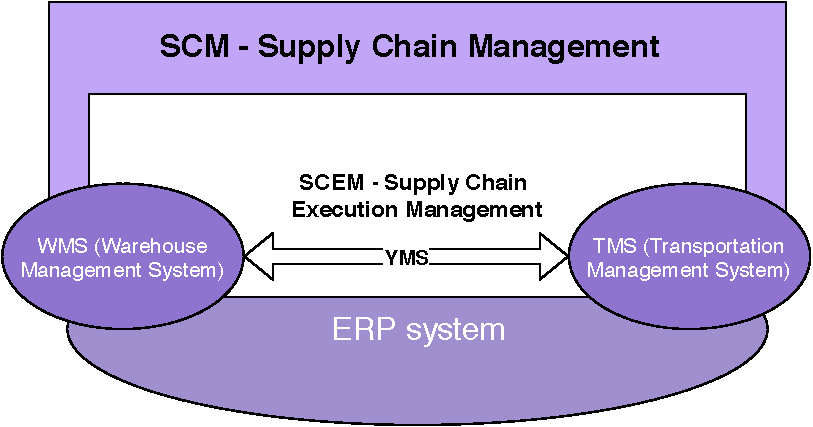
\includegraphics[width=0.9\linewidth,]{figure/tms_system} 

}

\caption{TMS in the Supply Chain Management Information System}\label{fig:tms}
\end{figure}
\hypertarget{obstacles-in-strategic-planning-of-rd-at-industrial-enterprises}{%
\chapter{Obstacles in strategic planning of R\&D at industrial enterprises}\label{obstacles-in-strategic-planning-of-rd-at-industrial-enterprises}}

In the rapidly developing post-industrial economy, a key factor in the effectiveness of doing business in high-tech industries, including in the transportation systems, is innovative activity based on scientific achievements and the practical implementation of these achievements. The potential of intangible assets of an enterprise is directly related to the competitiveness of a high-tech enterprise. The costs of research and development (R\&D) of world leaders in high-tech industries are measured in billions of dollars and euros. The logistics sector of the global economy and its' scientific and industrial base are often considered as one of the main engines of technological progress. This became apparent back at the beginning of the 21st century when there was an emerging need for fleet operations. Currently, the industry is developing dynamically and stably, which is primarily due to the processes in disruptive technologies in the automotive industry and the era of new mobility services under the circumstances of the digital economy. Research (2018) researches reported that the global market for fleet management systems in 2017 was USD 11.9 trillion and that by 2024, the global market is expected to reach USD 43.5 trillion, at CAGR of around 20.3 percent between 2018 and 2024. Thus, the technological development and the level of competitiveness of a company operating in high technology industries, including the fleet industry largely depends on the effectiveness of its scientific and technical activities and patent activity (Roy, 2013, @phelpsPatentsReallyPromote). The technical level of high-tech products is ensured, among other factors, by the degree of legal protection of the technologies underlying it, since the legal protection of products gives the enterprise a legal monopoly on its production and sale in the countries where the patent is valid.

Intellectual property (IP) rights are a special type of property, which is characterized by both characteristics related to tangible property and a number of specific properties. Among the characteristics relating to both material and intellectual property, the following can be distinguished:
\begin{itemize}
\tightlist
\item
  the possibility of carrying out such legal operations as purchase and sale, leasing, gratuitous transfer with the property;
\item
  the owner has the right to prevent the unauthorized use or sale of the property.
\end{itemize}
The main differences of intellectual property are immaterial and inexhaustibility. The inexhaustibility of intellectual property means that the rights to it cannot be alienated mechanically, as its carrier, for example, a flash drive with a program recorded on it. It is possible only with the help of the legislative mechanism to prohibit an individual or legal entity from using a specific scientific and technological achievement, access to which this person received legally or illegally. The system of protecting the results of intellectual activity existing in the world today not only gives the creators of innovations significant competitive advantages, but also poses a number of serious problems for them. One of these problems is patent wars. Figure \ref{fig:numberofpatents} represents increasing number of patents during period from 1990 to 2017.
\begin{figure}[h]

{\centering 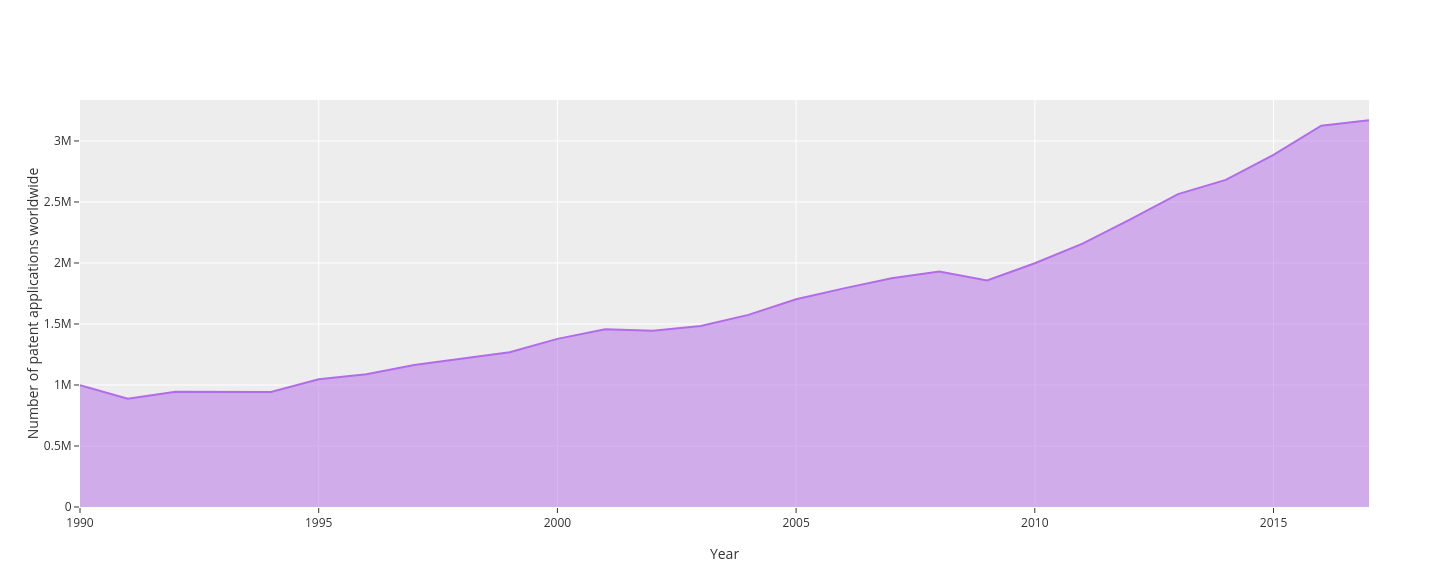
\includegraphics[width=0.9\linewidth,]{figure/Numberofpatents} 

}

\caption{Number of patents}\label{fig:numberofpatents}
\end{figure}
One of the strategies used by companies in patent wars is the use of blocking patents, which are a specific technological area and prevent the use of other patents in it. Patents are also widely used to protect the maximum number of technical solutions within a single document. As noted above, one of the key factors for successful innovation is the focus of R\&D on the creation of promising results of intellectual activity. In the market of high-tech products, usually it is the presence of finalized results of intellectual activity that provides most of the added value to the product and resulting in high profits. In addition, patent protection allows you to bring products to the world market and makes them competitive.The terms of reference for the development of new products are mainly focused not on current trends in the development of the fleet industry, but on the actual capabilities of enterprises. The key to high competitiveness in these conditions is the effective implementation of R\&D, leading to the creation of patentable scientific and technical solutions with world novelty, since patenting of developments provides the company with a natural monopoly. Fleet enterprises have high scientific and technical potential, which is often not fully realized due to inefficient management and R\&D planning, which is not aimed at creating patentable technologies and, as a result, does not allow companies to compete at the global level and effectively solve social and economic problems.

Planning is one of the five management functions formulated by A. Fayol and implies as setting goals, finding ways to achieve them and determining the directions in which the company should move. Planning provides the basis for other functions that, in turn, are focused on the implementation of the plans of the organization (Vliet, 2014).

Depending on the goals of planning, baseline information, regulatory framework and final planned indicators, various planning methods are used. The paper considers the classification of planning methods according to the stages of the development of plans, presented in Figure 1.12. Depending on the goals of planning, strategic planning, tactical (business planning) and operational planning are distinguished (Misni \& Lee, 2017). According to the work of X, strategic planning is a set of actions and decisions of the leader leading to the development of specific strategies designed to achieve the goals of the company, and the strategy includes the entire set of global ideas for the development of the company, and not just focused on a specific period. P. Lorange describes the strategic planning process as a tool to help make management decisions and ensure innovations and changes in the company. He identifies four main types of management activities in the strategic planning process:
\begin{itemize}
\tightlist
\item
  Resource allocation
\item
  Adaptation to the external environment
\item
  Internal coordination
\item
  Organizational strategic foresight
\end{itemize}
Concerning the research of (Meyersdorf \& Dori, 1997) that R\&D is a dynamic control object, and therefore any R\&D planning system must have the flexibility and mechanism for continuous analysis of incoming information that ensures sound management decisions throught object-process analysis (OPA). According to numerous works - planning of innovation and investment activities, including the organization of R\&D, should be considered in the overall system of strategic planning and management of the organization, which implies the application of the following principles of strategic planning of innovation:
\begin{enumerate}
\def\labelenumi{\arabic{enumi}.}
\tightlist
\item
  The principle of consistency, providing communication of all aspects of management activities.
\item
  Scientific principle, ensuring the development of methods and tools for managing innovation.
\item
  The principle of flexibility, which implies the ability of the company to quickly respond to changes in the external and internal environment.
\item
  The principle of selection of qualified personnel, ensuring the effectiveness of innovation at all levels.
\item
  The principle of risk minimization in the management of innovative investment projects.
\item
  The principle of ensuring the competitiveness of created innovative products.
\item
  The principle of obtaining maximum income with minimum investment.
\end{enumerate}
Taking into account these principles, the company's innovation strategy is a set of measures by the management to develop innovative ideas and concepts in the implementation of innovation and investment projects in accordance with the goals and objectives of this company. The methods of strategic planning in high-tech industrial enterprises are explored in several academic works and the system of economic indicators is examined to ensure long-term goal-setting and scenarios of innovative strategies in the high-tech industry.

From the standpoint of the concept of knowledge management, the strategic planning of scientific and technical programs of organizations is considered. A comprehensive scientific and technical program is defined as a form of organization of research and development in a company aimed at a single result. The program provides for the development, production and use of high-tech products and is a set of innovative projects that are united in purpose, themes, deadlines and funding mechanism.

Strategic planning methods for small high-tech industrial enterprises are studied in by Berry (1998); in particular, the author considers a system of economic indicators to ensure long-term goal-setting and innovative strategy scenarios in the high-tech industry. From the standpoint of the concept of knowledge management some researchers consider the strategic planning of scientific and technical programs of organizations. A comprehensive scientific and technical program is defined by the authors as a form of organization of research and development in the company aimed at a single result. The program provides for the development, production and application of high technology products and represents a set of innovative projects that are combined by purpose, subject, deadlines and financing mechanism (Shannak, Masa'deh, \& Akour, 2012).

The most important functions of the strategic planning of scientific and technical programs are:
\begin{enumerate}
\def\labelenumi{\arabic{enumi}.}
\tightlist
\item
  Information support for developers, investors and organizers in the form of strategic data bases relating to environmental conditions that affect strategic decisions in the organization.
\item
  Analytical activity that allows you to assess the current situation, make assumptions about the most likely areas of scientific and technical development of the future and choose the structure of the program, the principles of its implementation, requirements for program participants.
\item
  Prediction of the scientific and technological development of the country's economy in the field of the program being formed in order to study alternative development options.
\item
  Technical and economic function, consisting in the development of a system of plans containing all types of planned indicators at the end of the corresponding period.
\end{enumerate}
Nieto (2003) in his work considers innovation management as one of the tasks of strategic management of the company, which can be view from the position of macro and micro changes related to technological innovation (TI) within different economic units.

Strategic planning methods at high-tech industrial enterprises are studied by multiple authors (Berry, 1998, @ernstIntegratedPortfolioApproach2003, @kangReviewTechnologyForecasting2013); in particular, the authors consider a system of economic indicators to ensure long-term goal-setting and scenarios of innovative strategies in the high-tech industry.

From the standpoint of the concept of knowledge management in Trappey \& Trappey (2008) consider the strategic planning of scientific and technical programs of organizations. A comprehensive scientific and technical program is defined by the authors as a form of organization of research and development in the company aimed at a single result. The program provides for the development, production and application of high technology products and represents a set of innovative projects that are combined by purpose, subject, deadlines and financing mechanism.

G.Ya. Goldstein in {[}37, p.~68{]} considers innovation management as one of the strategic management objectives of the company, however, he notes that the R\&D sphere, despite the many-sided relations with other areas of the organization's activity, is usually relatively isolated, due to the uncertainty of the R\&D process and the specifics of R\&D activities. This factor, according to the author, provides a ``managerial gap'' between the positions and motivation of R\&D leaders and other managers, which, in turn, determines the problems of managing the R\&D process in the areas of marketing approach to R\&D, R\&D strategies as part of a firm's overall strategy and etc. A functional analysis of the intellectual property management process is given in the work of DB Shulgina and N.A. Shulginoy {[}41{]}. Features of the R\&D management sphere are also considered in {[}42, C. 274-277{]}. In accordance with these features, according to the author, the R\&D planning system should include a flexible system for monitoring the actual state of work and a mathematical apparatus for assessing the situation, as well as be linked to objective methods of scientific and technical forecasting and a system of feasibility studies for ongoing projects {[}{]}.

Within the framework of this method, the tasks and methods of thematic R\&D planning are of great importance. Portfolio is formed on the basis of industrial competition, comprehensive targeted scientific and technical programs and forecasts, direct contracts with customers and initiative proposals of researchers and developers. However, the scientific feasibility of thematic R\&D planning can only be ensured by fulfilling the following conditions:
\begin{itemize}
\tightlist
\item
  identification of promising ideas and research directions in the field of technology;
\item
  the introduction of scientifically based methods for assessing the scientific and technical level and the effectiveness of the created equipment;
\item
  development of a system of qualitative and quantitative assessment;
\item
  development of a mathematical model for determining the priority of topics;
\end{itemize}
Also, thematic planning should take into account economic criterias such as internal rate of return, profitability index, development costs, payback period, expected sales, etc. To assess the novelty of the development, the criteria of prospects, patentability, scientific and technical level, etc. are used.

Tactical planning for the goals set by the strategy determines the appropriate measures for the development of the enterprise. The task of tactical planning is to ensure the implementation of the strategic plan by choosing alternative options for achieving goals, their economic evaluation, determining criteria for choosing the best option. In the tactical planning of innovation and investment activities, business plans for future projects are developed, which substantiate all aspects of the use of investment resources and ensuring the technical level of new products {[}{]}. I.G. Shurygina in {[}43{]} analyzes the existing methods for evaluating R\&D projects that are used in the management and planning of R\&D, notes the importance of an approach to project evaluation based on competitiveness, and offers a model of the R\&D project management mechanism presented in Figure 1.14. Thus, one of the tools for strategic planning of R\&D is scientific and technical forecasting.

The methodologies of scientific and technical forecasting were studied by the works of J. Martino, E. Yancha, R. Aires, S. Sargsyan, N.I. Komkova, G.G. Balayan, B. Twiss and other scientists.

In {[}49{]}, the classification of types of forecasts and corresponding methods, presented in Figure 1.15, was considered.

Thus, one of the tools for strategic planning of R\&D is scientific and technical forecasting.

The methodologies of scientific and technical forecasting were studied by the works of J. Martino, E. Yancha, R. Aires, S. Sargsyan, N.I. Komkova, G.G. Balayan, B. Twiss and other scientists.

In {[}49{]}, the classification of types of forecasts and corresponding methods, presented in Figure 1.15, was considered.

Foresight-type forecasting methods are widely used, which involve the study of the development prospects of markets and industries for the production of high-tech products and the substantiation of managerial decisions {[}49, 50{]}. The Technology Assessment (TA) methodology provides for a combination of technological development monitoring and forward-looking assessments and develops mainly in the direction of social and political choice related to technological development.
Strategic Intelligence is a knowledge-based decision tool. In the scientific and industrial environment, traditional technology forecasting is most applicable. In domestic practice, as the author notes {[}50{]}, complex forecasts combining different types are mainly used.

Technological forecasting differs from the economic and socio-economic uncertainty of the content and characteristics of the object in the future. This uncertainty is overcome by using methods of high-quality forecasting, in particular, methods of target management and information-logical models. The basis of information-logical models are phased and hierarchical models.

Phased models are formed by constructing successive states of the predicted object from the initial state to the final one, which is determined by the development goals of the object. Figure \ref{fig:forecastingmethods}.
\begin{figure}[h]

{\centering 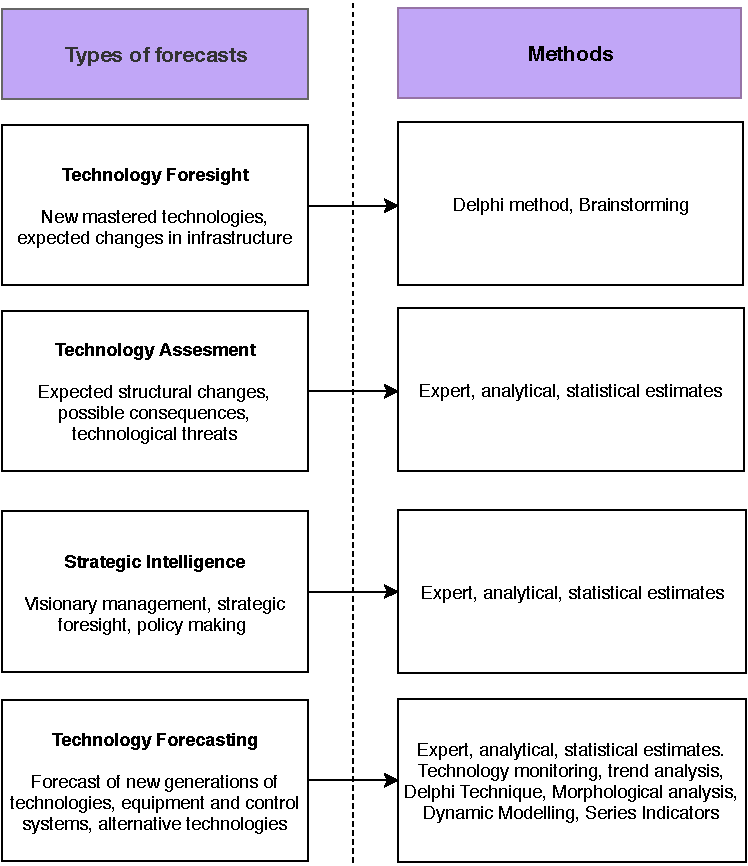
\includegraphics[width=0.9\linewidth,]{figure/forecasting_methods} 

}

\caption{Classification of types of forecasts}\label{fig:forecastingmethods}
\end{figure}
Hierarchical models consider development prospects at different levels of detail and are most often presented in the form of a ``goal tree''. The following classification of technological forecasting methods is given in {[}50{]}:
\begin{itemize}
\tightlist
\item
  qualitative methods
\item
  survey work
\end{itemize}
Methods by which new technological information is generated (extrapolation method, morphological study, scenario method);

Methods by which the available technological information is ordered and processed (historical analogy, scenario method, probabilistic transformation methods, operational models). There are such approaches as normative methods (such as network methods and system analysis). However, it should be noted that many traditional methods of scientific and technical forecasting are more focused on the industry level and less applicable for forecasting at the micro level. In {[}51{]} it is noted that the dynamic development of high-tech enterprises requires the improvement of methodological foundations and tools for predicting their development. The issues of technological forecasting and determining product requirements based on patent research in their works are considered by E.P. Skornyakov, M.E. Gorbunova, L.G. Kravets.

The prognostic potential of patent information is associated with two factors {[}52, C. 18{]}:
\begin{enumerate}
\def\labelenumi{\arabic{enumi}.}
\item
  The outstripping nature of patent information - it becomes available to a wide circle of users several years before the appearance of the corresponding products on the market.
\item
  A direct relationship between the intensity of patenting and the cost of R\&D associated with the creation and improvement of products.
\end{enumerate}
One of the most effective methods for analyzing trends in the development of scientific and technical areas related to the improvement of a product is the method of analyzing inventive activity, based on the assumption that a constant increase in R\&D costs leads to an increase in inventive activity associated with the development of this direction {[}52 , C. 26{]}.

In {[}53, C. 57{]}, the authors note that the description of the invention contains a section that analyzes the previous state of development of an object of technology and formulates requirements for improving this object. The analysis of this section allows you to compile a list of technical requirements for the product, since the technical requirements formulated by the inventors largely reflect the real requirements of consumers. Thus, the analysis of patent information significantly complements the traditional methods for identifying product requirements based on questionnaires and surveys.

Based on the foregoing, it can be concluded that R\&D planning is an integral part of the innovation management system in a high-tech company and is carried out at strategic, tactical and operational levels. The objective of strategic R\&D planning is to substantiate the subject of R\&D in the long term, taking into account the results of scientific and technical forecasting and patent research, tactical planning ensures the direct formation of the R\&D portfolio within existing resources; operational planning of R\&D provides a refinement of the system of indicators identified at the stage of tactical planning.

\clearpage

\hypertarget{technology-assessment-and-theoretical-framework}{%
\chapter{Technology Assessment and Theoretical framework}\label{technology-assessment-and-theoretical-framework}}

\hypertarget{innovation-concept}{%
\section{Innovation concept}\label{innovation-concept}}

There are various of rick and uncertainties that can be faced in innovative organization. Innovation is associated with the uncertainty of the economic situation arising from the volatility of supply and demand for goods, money, factors of production, from the multivariance of areas of capital investment and the diversity of criteria for the preference of investing, from limited knowledge about business and commerce and many other circumstances. In my opinion, uncertainty in innovation and innovation risks refers to the likelihood of losses arising when an entrepreneurial firm invests in the production of new goods or servants, in the development of new equipment and technologies that may not find the expected demand in the market, and also when investing in the development of managerial innovations that are not will bring the expected effect. The eight major factor shown in the Figure @ref(fig:innovationpractices., formulated on reviewed literature.
\begin{figure}[h]

{\centering 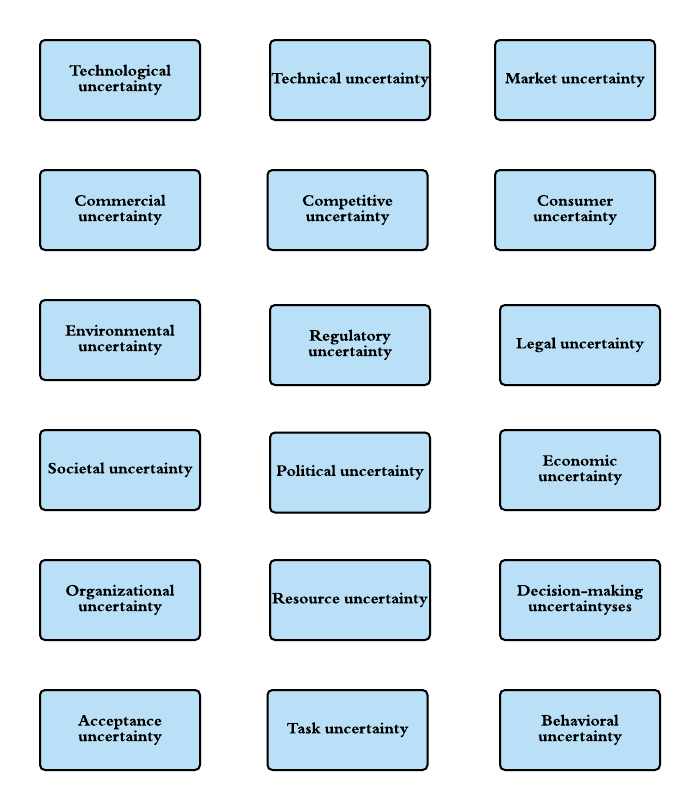
\includegraphics[width=0.8\linewidth,]{figure/4} 

}

\caption{Various authorities of uncertainty in innovation practices. Adopted from Jalonen (2011)}\label{fig:innovationpractices}
\end{figure}
For the NPD success factors there is a table summarizing each of the notions in for of the table for the common success factors must-know objectives (as shown in Table 1.). One of the most important factor, that most authors point out about cross-functional integration and this factor correlates with the installation about the nature of the NPD project - its implementation affects several functional processes of the company, including marketing, research and development, production, etc. (Schimmoeller, 2010).

The proposed grouping divides the totality of NPD project success factors into 4 groups:
* Developed strategy
* Features of the company
* New product development processes
* External factors

Basically, diffusion of managerial innovation is the transfer of managerial technology and organizational innovation showed in Figure \ref{fig:seven}.
\begin{figure}[h]

{\centering 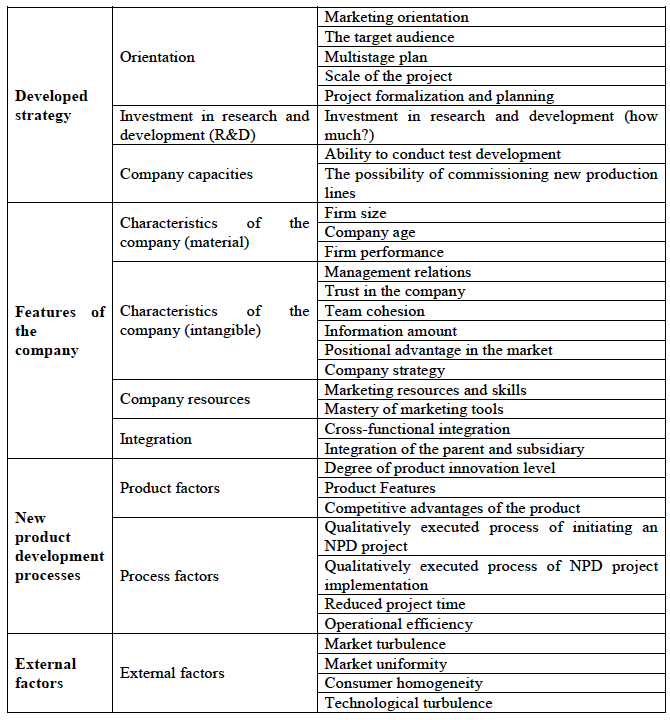
\includegraphics[width=0.7\linewidth,]{figure/7} 

}

\caption{Self-made table based on article of the Lee Schimmoeller, combined with additional thoughts (2010)}\label{fig:seven}
\end{figure}
\hypertarget{innovation-outputs}{%
\section{Innovation outputs}\label{innovation-outputs}}

At first, it is essential to have a full description of 4P's innovation theoretical concept. The original notion of the ``innovation'' itself the term of ``innovations'' were first used at the beginning of the 20th century by the well-known economist Joseph Schumpeter as specific term in order to designate and use new types of consumer goods, new production and vehicles, markets and forms of organization in industry working on new principles (Śledzik, 2013). Beforehand, it is vital to cover four major topics such as definitions of innovation, creating and capturing value from innovation, innovation, and performance and models of innovation. Considering different characteristics of each of those, 4P's model consists of directions of change: product innovation, process innovation, position innovation and paradigm innovation respectively and within this framework, innovation can be described as ``radical'' and ``incremental'' depending on the components and architecture. Without revising old models and trying to analyze new concepts, effective management and understanding are impossible. Organizational structure notion itself, innovation-oriented business culture and competencies are vital aspects which lead innovative enchacment (Bessant \& Tidd, 2013). So, such narrative has core value for innovation theory, and it is precisely described in the paper of Francis \& Bessant (2005).
Figure \ref{fig:mindmap} is representing Innovation paradigm schematic mind map.
\begin{figure}[h]

{\centering 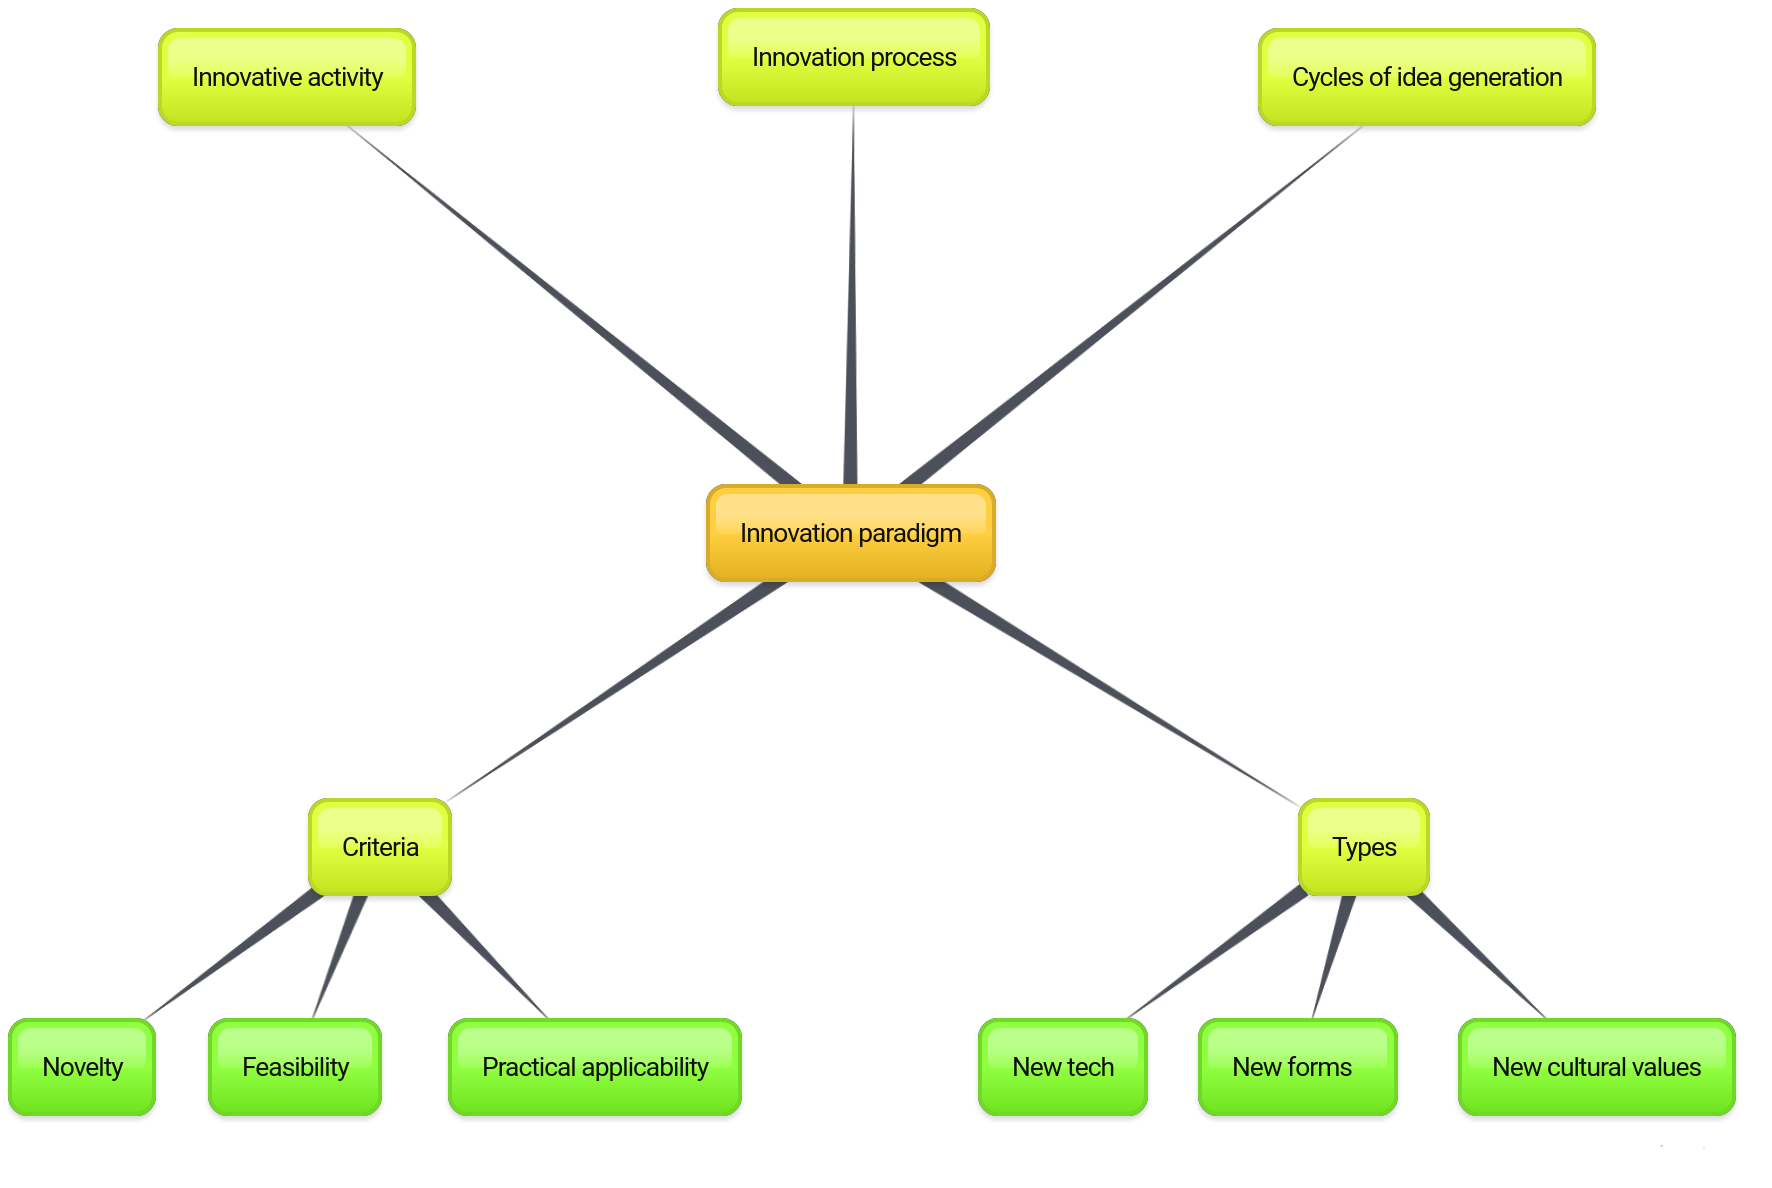
\includegraphics[width=0.8\linewidth,]{figure/1} 

}

\caption{Innovation paradigm schematic mind map}\label{fig:mindmap}
\end{figure}
\hypertarget{key-components-of-the-innovative-organization}{%
\section{Key components of the innovative organization}\label{key-components-of-the-innovative-organization}}

From the standpoint of the organization, the following are traditionally considered as the main elements of innovation activity, such as defining management objectives, strategy development, analysis and evaluation of particular management effectiveness (KPIs), adjustment of innovation processes, organization of monitoring the implementation of the program of innovation activities, additional coordination of the program implementation, definitions of control technologies, management program development.

Innovation process proposes to understand a consistent chain of events in which innovations mature from the idea to a specific product, technology or service and are considered in economic practice. Most of them described in research conducted by Joe Tidd and related to the leadership capabilities and building innovation culture among employees as well as needs of further characterisations and higher complexity in technological, market and organisational contingencies and internal assets R\&D activities (Tidd, 1997). Figure \ref{fig:components} showing . Some research is devoted to (Matthews, 2003).

Followed by the concept of ``high-involvement innovation'' (HII), we can differentiate between different stages of evolution of development and characteristics related to them (five-stages model). Generally, it relies upon the field of the continuous improvement (CI) through mobilising a high level of involvement of the workforce in sustained incremental innovation, and some of their effects (Bessant \& Caffyn, 1997). Thus, this might result in increased performance of an organization through the implementation of ``high-involvement innovation'' and amenable atmosphere for people to change. There is also a correlation between HII and HR performances, based on the promotion of employee involvement in the industry (Bondarev \& Zashchitina, 2017).

Finally, the ``SPOT'' framework stands as shift model from traditional strategy to the strategic innovation approach. Three of the letters describe different processes: P -- Innovation Processes, O -- Organization for
4 innovation, T -- Tools \& Technologies to support innovation (abbreviation). Essential ``must-know'' was about innovation culture and creative climate (analyze of the innovative organisation should take in account disciplines and normative/descriptive approaches). For the fleet services management, utalization of innovational approaches could be seen in the data transfer in product manufacturing installation base.
\begin{figure}[h]

{\centering 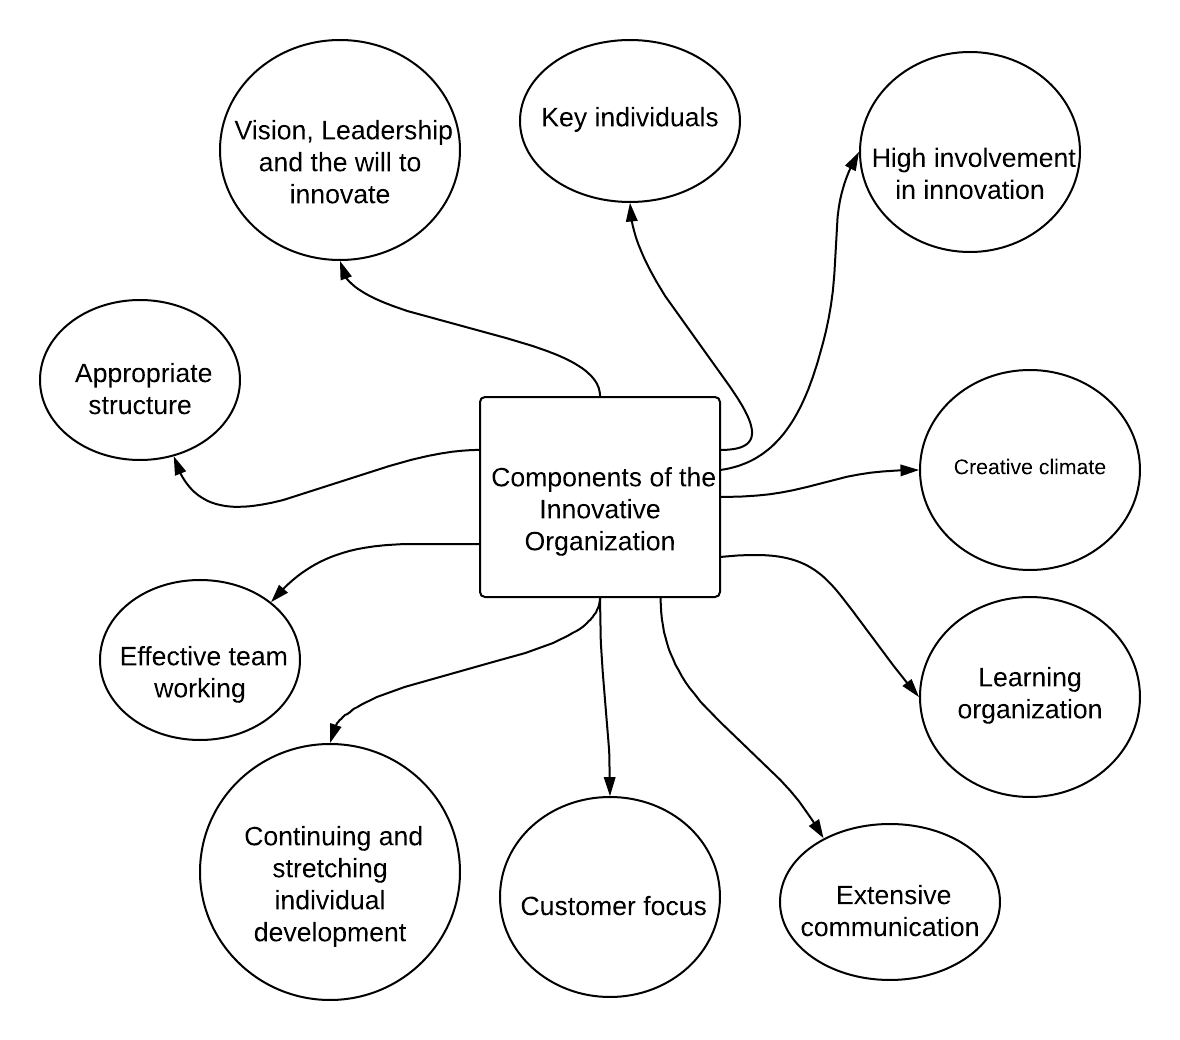
\includegraphics[width=0.8\linewidth,]{figure/2} 

}

\caption{Components of the innovative organization}\label{fig:components}
\end{figure}
\hypertarget{development-of-innovation-strategy}{%
\section{Development of innovation strategy}\label{development-of-innovation-strategy}}

Case studies have been long established in innovation strategy to present a detailed analysis of the capabilities approach. Meanwhile, the was a representation of the key factors in innovation strategy structuring and several cognitive limits affecting movement to a distinct path. However, we have to mention about Dynamic capabilities, so it may be considered as the company's ability to undertake volatile environment's changes and productively use existing resources for creating new configurations of routines and resources. Though the concept of dynamic capabilities is comprehensive enough the core definitions of current concept point to the various organizational processes, such as integration, learning, modification, and others. The paper {[}34, C. 92{]} provides a classification of innovative strategies, presented in Figure 1.16, in which strategies focused on active innovative activity are combined into a group of technological ones. At the same time, the creation of fundamentally new technologies involves only a leadership strategy and, to a somewhat lesser extent, a strategy for following the leader, implying a thorough study and fundamental improvement of products created by competitors. The remaining strategies (imitations, copying, dependencies and improvements) are not focused on the full use of the company's own innovative and technological potential. All these strategies can allow the company to compete effectively in certain markets and get a satisfactory financial result, but most of them are not able to ensure the company's competitiveness in the long run
\begin{figure}[h]

{\centering 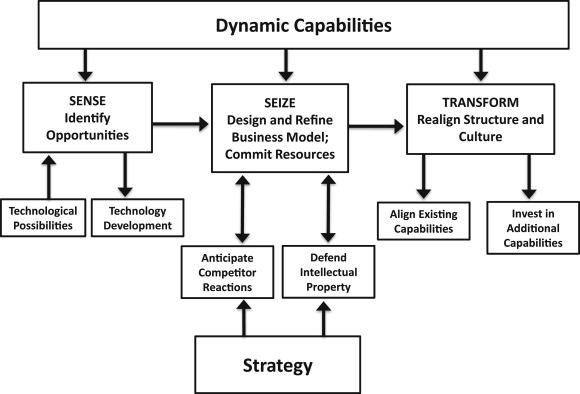
\includegraphics[width=0.8\linewidth,]{figure/3} 

}

\caption{Dynamic capabilities as refinery for business model. Source from Treece (2018)}\label{fig:unnamed-chunk-2}
\end{figure}
\hypertarget{literature-review-on-creativity-principles}{%
\section{Literature review on creativity principles}\label{literature-review-on-creativity-principles}}

At the moment there are many tools for generating ideas based primarily on the development of creative thinking and team searching for a concrete solution, which usually coming along with usage of heuristic methods to quicklycer ``work out'' and select many options for the subsequent creation of a product or the solution of problems. However, most scholars do not have equal concensus on management application, generating ideas and ideation that would foster innovative potential and affected productivity and capacity within firms' boundaries in certain way (Dorow, Davila, Varvakis, \& Vallejos, 2015).

The terminology related to ideas generation is described in details in the works of A.Kraslawski, namely, the application of the TRIZ methodology in engineering tasks and product development task segmentation tequinieqs, such as morphological analysis, analogy methods, synectics, brainstorming and lateral thinking (Srinivasan \& Kraslawski, 2006). Although these tools and methods have temporary advantages and make it possible to evaluate the problem from various angles, the experience of the team members serves as the basis for their implementation and should be considered within whole problem structure and. Explicitly, the patent research and patent analysis belong to group of search tools, gaining valuable insights throught new solutions, which is the key to the success of any ongoing project, especially in fleet management, where recent technologies play huge role in gaining advantage on the market. Systematic creativity and innentive principles posses great amount of impact to the scientific, engineering and business tasks and various applications (Mann \& Dewulf, n.d.).

Analysis of patent information is also considered a tool for finding innovative solutuions, while the inventors often underestimate as valuable tool. This trend, to a greater extent, is a consequence of the fact that when conducting patent research, many experts use a limited set of tools to find a new solution.

In particular, the most common tool for such purposes is the construction of the semantic and topological patent graphs matrix and mapping patent classification, which, of course, makes it possible to visualize all the main technical directions of the research object development in a visual and compact form, but mainly aims at systematization of relevant information (Yan \& Luo, n.d., @officeCooperativePatentClassification). Therefore, it does not allow to fully disclose the application potential of patent information for inventors.

\hypertarget{the-technology-life-cycle-and-major-concepts}{%
\chapter{The technology life cycle and major concepts}\label{the-technology-life-cycle-and-major-concepts}}

\hypertarget{s-curves-as-models-of-innovation}{%
\subsection{S-curves as models of innovation}\label{s-curves-as-models-of-innovation}}

Applying mathematical princepls within managerial framework gives abbility to predict flow of innovation life cycle and form an accurate innovation model. Hence, over time the performance of any system andthe value of its main production function naturally changes. Dynamics of a certain evolving indicator goes through several stages in its development. These changes are described by an empirical dependence, having the form of a stylized S-shaped curve. These changes are described by an empirical dependence, having the form of a stylized S-shaped curve. By using the S-shaped curve we can visualize the processes of transition of a socio-economic system from one stable state to another, processes of radical changes accompanying its innovative activity as well as processes of growth and development during crisis stage and other phenomenas. The practical application of the logistic S-shaped curve in the study of innovation was investigated by Foster (1986). The concept of technology S-curves suggests that the amount of improvement in the characteristics of a product or technology over a given period of time or due to a given volume of intellectual costs changes as it grows older/mature. In the early stages of development, product quality improves relatively slowly. With the development of technology, the pace of technological improvement is growing. However, at the stages of maturity, the technology will asymptotically approach the natural or physical limit and for further improvements more and more intellectual and time costs will be needed. The essence of strategic technology management is to determine when the inflection point on the S-curve of technology has already been passed, and then identify and develop next-generation technologies that ultimately change the current one. Thus, the most important thing is to change the technology in time at the intersection point of the S-curves of the old and new technologies. According to the definition given in Kasztler et al. (2012), at the emergence stage, a new technology has practically no competitive influence and is poorly integrated into products or processes. During the period of ``growth'', the pace of technology diffusion accelerates, its competitiveness increases, while its integration into new products or processes is still small. Having reached ``maturity'', a number of common technologies acquire the status of key ones and integrate into products or processes, consolidating their high competitive potential. With the loss of competitive influence, the technology becomes basic, enters the saturation stage and can be replaced by new technology. As can be seen from Figure \ref{fig:scurve}, the most critical factors are Technology Limit and Change in Productivity Ratio. A change in productivity coefficient is defined as a turning point due to the emergence of a new opportunity. Another factor is the technological limit. This is manifested when the technology, having exhausted the potential for improvement, reaches maturity. It is at this level that process innovations often take place.
\begin{figure}[h]

{\centering 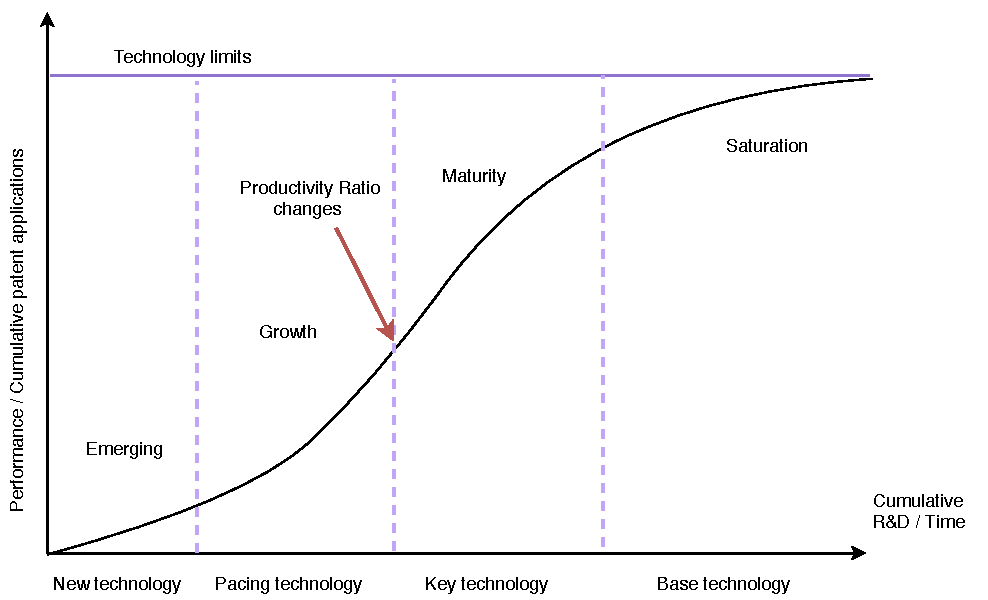
\includegraphics[width=0.8\linewidth,]{figure/S_curve} 

}

\caption{The S-curve concept of technology life cycle}\label{fig:scurve}
\end{figure}
S-curves are formed using a regression model that describes the non-linear relationship between the dependent variable (prediction object) and time. The most commonly used equation presented in Sepúlveda, Paternina, \& Suarez (2014) and outlined the relationship between invested in R\&D activities.
\begin{equation} 
  Y_{t}=\frac{L}{1+a\cdot e^{-b\cdot t} }
\end{equation}
where parameter ``a'' determines the position of the curve along the time axis, parameter ``b'' characterizes the steepness of the middle part of the curve (both responsible for location and curve shape). ``L'' characterizes the upper limit of growth (
asymptotic maximum of the function Y\textsubscript{2}). Currently, quite a lot of materials have been published in which the analysis of the S-curve is presented as a tool for describing and predicting the system development.

\hypertarget{patent-analysis}{%
\subsection{Patent analysis}\label{patent-analysis}}

From the standpoint of modern strategic mangament approaches, it is necessary to go on to consider the strategic justification of the patent method and directions of possible application areas. Despite the fact that technology is becoming the main competitive advantage in many markets, a number of managers and decision-makers still have insufficient information about the possible effects of technological changes on the competitiveness of their organization. Providing such missing information is the main function of patent analysis, the value of which lies in the ability to provide most of this information using bibliometric methods. Patent analysis uses bibliometry to analyze the set of data found in patent databases in order to identify leading indicators of technological change. The number of times that a patent is cited provides strategic information on which technologies reach critical mass. In addition, such an analysis determines which competitors and industries actively follow these technologies {[}WIPO{]}.

\hypertarget{tables-graphics-references-and-labels}{%
\chapter{Tables, Graphics, References, and Labels}\label{tables-graphics-references-and-labels}}

\hypertarget{tables}{%
\section{Tables}\label{tables}}

asda

\clearpage

\hypertarget{figures}{%
\section{Figures}\label{figures}}

\hypertarget{conclusion}{%
\chapter*{Conclusion}\label{conclusion}}
\addcontentsline{toc}{chapter}{Conclusion}

If we don't want Conclusion to have a chapter number next to it, we can add the \texttt{\{-\}} attribute.

\textbf{More info}

And here's some other random info: the first paragraph after a chapter title or section head \emph{shouldn't be} indented, because indents are to tell the reader that you're starting a new paragraph. Since that's obvious after a chapter or section title, proper typesetting doesn't add an indent there.

\appendix

\hypertarget{the-first-appendix}{%
\chapter{The First Appendix}\label{the-first-appendix}}

This first appendix includes all of the R chunks of code that were hidden throughout the document (using the \texttt{include\ =\ FALSE} chunk tag) to help with readibility and/or setup.

\textbf{In the main Rmd file}
\begin{Shaded}
\begin{Highlighting}[]
\CommentTok{# This chunk ensures that the thesisdown package is}
\CommentTok{# installed and loaded. This thesisdown package includes}
\CommentTok{# the template files for the thesis.}
\ControlFlowTok{if}\NormalTok{(}\OperatorTok{!}\KeywordTok{require}\NormalTok{(devtools))}
  \KeywordTok{install.packages}\NormalTok{(}\StringTok{"devtools"}\NormalTok{, }\DataTypeTok{repos =} \StringTok{"http://cran.rstudio.com"}\NormalTok{)}
\ControlFlowTok{if}\NormalTok{(}\OperatorTok{!}\KeywordTok{require}\NormalTok{(thesisdown))}
\NormalTok{  devtools}\OperatorTok{::}\KeywordTok{install_github}\NormalTok{(}\StringTok{"ismayc/thesisdown"}\NormalTok{)}
\KeywordTok{library}\NormalTok{(thesisdown)}
\end{Highlighting}
\end{Shaded}
\textbf{In Chapter \ref{ref-labels}:}

\hypertarget{the-second-appendix-for-fun}{%
\chapter{The Second Appendix, for Fun}\label{the-second-appendix-for-fun}}

\backmatter

\hypertarget{references}{%
\chapter*{References}\label{references}}
\addcontentsline{toc}{chapter}{References}

\markboth{References}{References}

\noindent

\setlength{\parindent}{-0.20in}
\setlength{\leftskip}{0.20in}
\setlength{\parskip}{8pt}

\hypertarget{refs}{}
\leavevmode\hypertarget{ref-berryStrategicPlanningSmall1998}{}%
Berry, M. (1998). Strategic planning in small high tech companies. \emph{Long Range Planning}, \emph{31}(3), 455--466. \url{http://doi.org/10.1016/S0024-6301(98)80012-5}

\leavevmode\hypertarget{ref-bessantHighInvolvementInnovationContinuous1997}{}%
Bessant, J., \& Caffyn, S. (1997). High-Involvement Innovation Through Continuous Improvement. \emph{International Journal of Technology Management - INT J TECHNOL MANAGE}, \emph{14}. \url{http://doi.org/10.1504/IJTM.1997.001705}

\leavevmode\hypertarget{ref-bessantManagingInnovation2013}{}%
Bessant, J., \& Tidd, J. (2013). \emph{Managing Innovation}.

\leavevmode\hypertarget{ref-bondarevHighInvolvementInnovation2017}{}%
Bondarev, M. G., \& Zashchitina, E. K. (2017). High involvement innovation: Analysing employee involvement and HR performance in the construction industry. In \emph{2017 International Conference "Quality Management,Transport and Information Security, Information Technologies" (IT QM IS)} (pp. 488--491). \url{http://doi.org/10.1109/ITMQIS.2017.8085868}

\leavevmode\hypertarget{ref-brockjohnsMagicQuadrantTransportation}{}%
Brock Johns, O. S. D. (n.d.). Magic Quadrant for Transportation Management Systems. Retrieved September 23, 2019, from \url{https://www.gartner.com/en/documents/3905867/magic-quadrant-for-transportation-management-systems}

\leavevmode\hypertarget{ref-dorowGenerationIdeasIdeation2015}{}%
Dorow, P., Davila, G. A., Varvakis, G., \& Vallejos, R. (2015). Generation of Ideas, Ideation and Idea Management. \emph{NAVUS - Revista de Gestão E Tecnologia}, \emph{5}, 51. \url{http://doi.org/10.18815/navus.v5i2.248}

\leavevmode\hypertarget{ref-ernstIntegratedPortfolioApproach2003}{}%
Ernst, H., \& Soll, J. (2003). An Integrated Portfolio Approach to Support Market-Oriented R\&D Planning. \emph{International Journal of Technology Management - INT J TECHNOL MANAGE}, \emph{26}. \url{http://doi.org/10.1504/IJTM.2003.003422}

\leavevmode\hypertarget{ref-fosterWorkingSCurveAssessing1986}{}%
Foster, R. N. (1986). Working The S-Curve: Assessing Technological Threats. \emph{Research Management}, \emph{29}(4), 17--20. \url{http://doi.org/10.1080/00345334.1986.11756976}

\leavevmode\hypertarget{ref-francisTargetingInnovationImplications2005}{}%
Francis, D., \& Bessant, J. (2005). Targeting innovation and implications for capability development. \emph{Technovation}, \emph{25}(3), 171--183. \url{http://doi.org/10.1016/j.technovation.2004.03.004}

\leavevmode\hypertarget{ref-griffisTransportationManagementSystems2007}{}%
Griffis, S., \& Goldsby, T. (2007). Transportation Management Systems: An Exploration of Progress and Future Prospects. \emph{Transportation}, \emph{18}, 18.

\leavevmode\hypertarget{ref-kangReviewTechnologyForecasting2013}{}%
Kang, D., Jang, W., Lee, H., \& No, H. J. (2013). A Review on Technology Forecasting Methods and Their Application Area, \emph{7}(4), 5.

\leavevmode\hypertarget{ref-kasztlerPracticesFutureRequirements2012}{}%
Kasztler, A., Apilo, T., Marcin, borowiecky, Budde, B., Karl-Heinz, leitner, Paasi, J., \ldots{} Zahradnik, G. (2012). \emph{Practices, future requirements and building blocks of a new innovation model}. \url{http://doi.org/10.13140/RG.2.2.21043.02086}

\leavevmode\hypertarget{ref-mannEvolvingWorldSystematic}{}%
Mann, D., \& Dewulf, S. (n.d.). Evolving The World's Systematic Creativity Methods, 10.

\leavevmode\hypertarget{ref-matthewsKnowledgeManagementInnovation2003}{}%
Matthews, J. H. (2003). Knowledge Management and Innovation: How are they related? In G. Timbrell (Ed.),. Presented at the KM Challenge 2003 Knowledge Management Conference, Melbourne Australia: Standards Australia. Retrieved from \url{https://eprints.qut.edu.au/14629/}

\leavevmode\hypertarget{ref-meyersdorfSystemModelingDomain1997}{}%
Meyersdorf, D., \& Dori, D. (1997). System modeling of the R\&D domain through the object-process methodology: A practical tool to help R\&D satisfy its customers' needs. \emph{R\&D Management}, \emph{27}, 333--344. \url{http://doi.org/10.1111/1467-9310.00069}

\leavevmode\hypertarget{ref-misniReviewStrategicTactical2017}{}%
Misni, F., \& Lee, L. S. (2017). A Review on Strategic, Tactical and Operational Decision Planning in Reverse Logistics of Green Supply Chain Network Design. \emph{Journal of Computer and Communications}, \emph{05}(08), 83--104. \url{http://doi.org/10.4236/jcc.2017.58007}

\leavevmode\hypertarget{ref-bartdemuynckMagicQuadrantTransportation2018}{}%
Muynck, B. D. (2018, March 19). Magic Quadrant for Transportation Management Systems. Retrieved September 27, 2019, from \url{https://www.gartner.com/en/documents/3869063}

\leavevmode\hypertarget{ref-nettstraterLogisticsSoftwareSystems2015}{}%
Nettsträter, A., Geißen, T., Witthaut, M., Ebel, D., \& Schoneboom, J. (2015). Logistics Software Systems and Functions: An Overview of ERP, WMS, TMS and SCM Systems. In (pp. 1--11). \url{http://doi.org/10.1007/978-3-319-13404-8_1}

\leavevmode\hypertarget{ref-nietoManagementKnowledgeManagement2003}{}%
Nieto, M. (2003). From R\&D management to knowledge management: An overview of studies of innovation management. \emph{Technological Forecasting and Social Change}, \emph{70}(2), 135--161. \url{http://doi.org/10.1016/S0040-1625(02)00196-8}

\leavevmode\hypertarget{ref-officeCooperativePatentClassification}{}%
Office, E. P. (n.d.). Cooperative Patent Classification (CPC). Retrieved May 25, 2019, from \url{https://www.epo.org/searching-for-patents/helpful-resources/first-time-here/classification/cpc.html}

\leavevmode\hypertarget{ref-phelpsPatentsReallyPromote}{}%
Phelps, M. (n.d.). Do Patents Really Promote Innovation? A Response To The Economist. Retrieved September 11, 2019, from \url{https://www.forbes.com/sites/marshallphelps/2015/09/16/do-patents-really-promote-innovation-a-response-to-the-economist/}

\leavevmode\hypertarget{ref-reportbuyerStrategicAnalysisFleeta}{}%
ReportBuyer. (n.d.). Strategic Analysis of Fleet Vehicle Leasing Market in Finland. Retrieved May 19, 2019, from \url{https://www.prnewswire.com/news-releases/strategic-analysis-of-fleet-vehicle-leasing-market-in-finland-300236544.html}

\leavevmode\hypertarget{ref-researchFleetManagementSystems2018}{}%
Research, Z. M. (2018, November 12). Fleet Management Systems Market Will Reach USD 43.5 Billion By 2024, Globally: Zion Market Research. Retrieved September 11, 2019, from \url{http://www.globenewswire.com/news-release/2018/12/11/1665175/0/en/Fleet-Management-Systems-Market-Will-Reach-USD-43-5-Billion-By-2024-Globally-Zion-Market-Research.html}

\leavevmode\hypertarget{ref-royIntellectualPropertyStrategy2013}{}%
Roy, D. (2013). Intellectual property strategy for competitive advantage. \emph{Int. J. Of Intellectual Property Management}, \emph{6}, 36--61. \url{http://doi.org/10.1504/IJIPM.2013.053449}

\leavevmode\hypertarget{ref-schimmoellerSUCCESSFACTORSNEW2010}{}%
Schimmoeller, L. (2010). SUCCESS FACTORS OF NEW PRODUCT DEVELOPMENT PROCESSES.

\leavevmode\hypertarget{ref-sepulvedaPatentApplicationsSource2014}{}%
Sepúlveda, J., Paternina, A., \& Suarez, A. (2014). Patent applications as source for measuring technological performance. \emph{Scientometrics}, \emph{98}(2), 1385--1395. \url{http://doi.org/10.1007/s11192-013-1050-4}

\leavevmode\hypertarget{ref-shannakKnowledgeManagementStrategy2012}{}%
Shannak, R., Masa'deh, R., \& Akour, M. (2012). Knowledge Management Strategy Building: Literature Review. \emph{European Scientific J.}, \emph{8}, 143--168.

\leavevmode\hypertarget{ref-srinivasanApplicationTRIZCreativity2006}{}%
Srinivasan, R., \& Kraslawski, A. (2006). Application of the TRIZ creativity enhancement approach to design of inherently safer chemical processes. \emph{Chemical Engineering and Processing: Process Intensification}, \emph{45}(6), 507--514. \url{http://doi.org/10.1016/j.cep.2005.11.009}

\leavevmode\hypertarget{ref-sledzikSchumpeterViewInnovation2013}{}%
Śledzik, K. (2013). Schumpeter's View on Innovation and Entrepreneurship. \emph{SSRN Electronic Journal}. \url{http://doi.org/10.2139/ssrn.2257783}

\leavevmode\hypertarget{ref-tiddComplexityNetworksLearning1997}{}%
Tidd, J. (1997). Complexity, Networks \& Learning: Integrative Themes for Research on Innovation Management. \emph{International Journal of Innovation Management}, \emph{01}(01), 1--21. \url{http://doi.org/10.1142/S1363919697000024}

\leavevmode\hypertarget{ref-trappeyKnowledgeManagementMethod2008}{}%
Trappey, A. J. C., \& Trappey, C. V. (2008). An R\&D knowledge management method for patent document summarization. \emph{Industrial Management \& Data Systems}. \url{http://doi.org/10.1108/02635570810847608}

\leavevmode\hypertarget{ref-alexandratwinWhyCompaniesUse}{}%
Twin, A. (n.d.). Why Companies Use Outsourcing. Retrieved June 1, 2019, from \url{https://www.investopedia.com/terms/o/outsourcing.asp}

\leavevmode\hypertarget{ref-vlietFiveFunctionsManagement2014}{}%
Vliet, V. van. (2014, June 23). Five Functions of Management by Henri Fayol. Retrieved May 25, 2019, from \url{https://www.toolshero.com/management/five-functions-of-management/}

\leavevmode\hypertarget{ref-WhatFleetManagement}{}%
What is fleet management? - Definition from WhatIs.Com. (n.d.). Retrieved June 1, 2019, from \url{https://whatis.techtarget.com/definition/fleet-management}

\leavevmode\hypertarget{ref-WhichOneYou2019}{}%
Which one is for you: TMS, FMS or Route Optimization Software? (2019). Retrieved October 6, 2019, from \url{https://www.abivin.com/single-post/2017/09/14/Which-one-is-for-you-TMS-FMS-or-Route-Optimization-Software}

\leavevmode\hypertarget{ref-wiyonoDESIGNINGELEARNINGMODEL2011}{}%
Wiyono, D., Pribadi, S., \& Permana, R. (2011). DESIGNING E-LEARNING MODEL TO LEARN ABOUT TRANSPORTATION MANAGEMENT SYSTEM TO SUPPORT SUPPLY CHAIN MANAGEMENT WITH SIMULATION PROBLEMS, \emph{6}. \url{http://doi.org/10.12777/jati.6.1.11-20}

\leavevmode\hypertarget{ref-yanMeasuringTechnologicalDistance}{}%
Yan, B., \& Luo, J. (n.d.). Measuring Technological Distance for Patent Mapping, 27.


% Index?

\end{document}
